%%%%%%%%%%%%%%%%%%%%%%%%%%%%%%%%%%%%%%%%%%%%%%%%%%%%%%%%%%%%%%%%%%%%%%%%
%%%%%%%%%%%%%%%%%%%%%% Simple LaTeX CV Template %%%%%%%%%%%%%%%%%%%%%%%%
%%%%%%%%%%%%%%%%%%%%%%%%%%%%%%%%%%%%%%%%%%%%%%%%%%%%%%%%%%%%%%%%%%%%%%%%

%%%%%%%%%%%%%%%%%%%%%%%%%%%%%%%%%%%%%%%%%%%%%%%%%%%%%%%%%%%%%%%%%%%%%%%%
%% NOTE: If you find that it says                                     %%
%%                                                                    %%
%%                           1 of ??                                  %%
%%                                                                    %%
%% at the bottom of your first page, this means that the AUX file     %%
%% was not available when you ran LaTeX on this source. Simply RERUN  %%
%% LaTeX to get the ``??'' replaced with the number of the last page  %%
%% of the document. The AUX file will be generated on the first run   %%
%% of LaTeX and used on the second run to fill in all of the          %%
%% references.                                                        %%
%%%%%%%%%%%%%%%%%%%%%%%%%%%%%%%%%%%%%%%%%%%%%%%%%%%%%%%%%%%%%%%%%%%%%%%%

%%%%%%%%%%%%%%%%%%%%%%%%%%%% Document Setup %%%%%%%%%%%%%%%%%%%%%%%%%%%%

% Don't like 10pt? Try 11pt or 12pt
\documentclass[10pt]{article}

% The automated optical recognition software used to digitize resume
% information works best with fonts that do not have serifs. This
% command uses a sans serif font throughout. Uncomment both lines (or at
% least the second) to restore a Roman font (i.e., a font with serifs).
%\usepackage{times}
%\renewcommand{\familydefault}{\sfdefault}

% This is a helpful package that puts math inside length specifications
\usepackage{calc}
\usepackage{comment}

% Simpler bibsection for CV sections
% (thanks to natbib for inspiration)
\makeatletter
\newlength{\bibhang}
\setlength{\bibhang}{1em} %1em}
\newlength{\bibsep}
 {\@listi \global\bibsep\itemsep \global\advance\bibsep by\parsep}
\newenvironment{bibsection}%
        {\begin{enumerate}{}{%
%        {\begin{list}{}{%
       \setlength{\leftmargin}{\bibhang}%
       \setlength{\itemindent}{-\leftmargin}%
       \setlength{\itemsep}{\bibsep}%
       \setlength{\parsep}{\z@}%
        \setlength{\partopsep}{0pt}%
        \setlength{\topsep}{0pt}}}
        {\end{enumerate}\vspace{-.6\baselineskip}}
%        {\end{list}\vspace{-.6\baselineskip}}
\makeatother

% Layout: Puts the section titles on left side of page
\reversemarginpar

%
%         PAPER SIZE, PAGE NUMBER, AND DOCUMENT LAYOUT NOTES:
%
% The next \usepackage line changes the layout for CV style section
% headings as marginal notes. It also sets up the paper size as either
% letter or A4. By default, letter was used. If A4 paper is desired,
% comment out the letterpaper lines and uncomment the a4paper lines.
%
% As you can see, the margin widths and section title widths can be
% easily adjusted.
%
% ALSO: Notice that the includefoot option can be commented OUT in order
% to put the PAGE NUMBER *IN* the bottom margin. This will make the
% effective text area larger.
%
% IF YOU WISH TO REMOVE THE ``of LASTPAGE'' next to each page number,
% see the note about the +LP and -LP lines below. Comment out the +LP
% and uncomment the -LP.
%
% IF YOU WISH TO REMOVE PAGE NUMBERS, be sure that the includefoot line
% is uncommented and ALSO uncomment the \pagestyle{empty} a few lines
% below.
%

%% Use these lines for letter-sized paper
\usepackage[paper=letterpaper,
            %includefoot, % Uncomment to put page number above margin
            marginparwidth=1.2in,     % Length of section titles
            marginparsep=.05in,       % Space between titles and text
            margin=1in,               % 1 inch margins
            includemp]{geometry}

%% Use these lines for A4-sized paper
%\usepackage[paper=a4paper,
%            %includefoot, % Uncomment to put page number above margin
%            marginparwidth=30.5mm,    % Length of section titles
%            marginparsep=1.5mm,       % Space between titles and text
%            margin=25mm,              % 25mm margins
%            includemp]{geometry}

%% More layout: Get rid of indenting throughout entire document
\setlength{\parindent}{0in}

\usepackage[shortlabels]{enumitem}

%% Reference the last page in the page number
%
% NOTE: comment the +LP line and uncomment the -LP line to have page
%       numbers without the ``of ##'' last page reference)
%
% NOTE: uncomment the \pagestyle{empty} line to get rid of all page
%       numbers (make sure includefoot is commented out above)
%
\usepackage{fancyhdr,lastpage}
\pagestyle{fancy}
%\pagestyle{empty}      % Uncomment this to get rid of page numbers
\fancyhf{}\renewcommand{\headrulewidth}{0pt}
\fancyfootoffset{\marginparsep+\marginparwidth}
\newlength{\footpageshift}
\setlength{\footpageshift}
          {0.5\textwidth+0.5\marginparsep+0.5\marginparwidth-2in}
\lfoot{\hspace{\footpageshift}%
       \parbox{4in}{\, \hfill %
                    \arabic{page} of \protect\pageref*{LastPage} % +LP
%                    \arabic{page}                               % -LP
                    \hfill \,}}

% Finally, give us PDF bookmarks
\usepackage{color,hyperref}
\definecolor{darkblue}{rgb}{0.0,0.0,0.3}
\hypersetup{colorlinks,breaklinks,
            linkcolor=darkblue,urlcolor=darkblue,
            anchorcolor=darkblue,citecolor=darkblue}

%%%%%%%%%%%%%%%%%%%%%%%% End Document Setup %%%%%%%%%%%%%%%%%%%%%%%%%%%%


%%%%%%%%%%%%%%%%%%%%%%%%%%% Helper Commands %%%%%%%%%%%%%%%%%%%%%%%%%%%%

% The title (name) with a horizontal rule under it
% (optional argument typesets an object right-justified across from name
%  as well)
%
% Usage: \makeheading{name}
%        OR
%        \makeheading[right_object]{name}
%
% Place at top of document. It should be the first thing.
% If ``right_object'' is provided in the square-braced optional
% argument, it will be right justified on the same line as ``name'' at
% the top of the CV. For example:
%
%       \makeheading[\emph{Curriculum vitae}]{Your Name}
%
% will put an emphasized ``Curriculum vitae'' at the top of the document
% as a title. Likewise, a picture could be included:
%
%   \makeheading[\includegraphics[height=1.5in]{my_picutre}]{Your Name}
%
% the picture will be flush right across from the name.
\newcommand{\makeheading}[2][]%
        {\hspace*{-\marginparsep minus \marginparwidth}%
         \begin{minipage}[t]{\textwidth+\marginparwidth+\marginparsep}%
             {\large \bfseries #2 \hfill #1}\\[-0.15\baselineskip]%
                 \rule{\columnwidth}{1pt}%
         \end{minipage}}

% The section headings
%
% Usage: \section{section name}
\renewcommand{\section}[1]{\pagebreak[3]%
    \hyphenpenalty=10000%
    \vspace{1.3\baselineskip}%
    \phantomsection\addcontentsline{toc}{section}{#1}%
    \noindent\llap{\scshape\smash{\parbox[t]{\marginparwidth}{\raggedright #1}}}%
    \vspace{-\baselineskip}\par}

% An itemize-style list with lots of space between items
\newenvironment{outerlist}[1][\enskip\textbullet]%
        {\begin{itemize}[#1,leftmargin=*]}{\end{itemize}%
         \vspace{-.6\baselineskip}}

% An environment IDENTICAL to outerlist that has better pre-list spacing
% when used as the first thing in a \section
\newenvironment{lonelist}[1][\enskip\textbullet]%
        {\begin{list}{#1}{%
        \setlength{\partopsep}{0pt}%
        \setlength{\topsep}{0pt}}}
        {\end{list}\vspace{-.6\baselineskip}}

% An itemize-style list with little space between items
\newenvironment{innerlist}[1][\enskip\textbullet]%
        {\begin{itemize}[#1,leftmargin=*,parsep=0pt,itemsep=0pt,topsep=0pt,partopsep=0pt]}
        {\end{itemize}}

% An environment IDENTICAL to innerlist that has better pre-list spacing
% when used as the first thing in a \section
\newenvironment{loneinnerlist}[1][\enskip\textbullet]%
        {\begin{itemize}[#1,leftmargin=*,parsep=0pt,itemsep=0pt,topsep=0pt,partopsep=0pt]}
        {\end{itemize}\vspace{-.6\baselineskip}}

% To add some paragraph space between lines.
% This also tells LaTeX to preferably break a page on one of these gaps
% if there is a needed pagebreak nearby.
\newcommand{\blankline}{\quad\pagebreak[3]}
\newcommand{\halfblankline}{\quad\vspace{-0.5\baselineskip}\pagebreak[3]}

% Uses hyperref to link DOI
\newcommand\doilink[1]{\href{http://dx.doi.org/#1}{#1}}
\newcommand\doi[1]{doi:\doilink{#1}}

% For \url{SOME_URL}, links SOME_URL to the url SOME_URL
\providecommand*\url[1]{\href{#1}{#1}}
% Same as above, but pretty-prints SOME_URL in teletype fixed-width font
\renewcommand*\url[1]{\href{#1}{\texttt{#1}}}

% For \email{ADDRESS}, links ADDRESS to the url mailto:ADDRESS
\providecommand*\email[1]{\href{mailto:#1}{#1}}
% Same as above, but pretty-prints ADDRESS in teletype fixed-width font
%\renewcommand*\email[1]{\href{mailto:#1}{\texttt{#1}}}

%\providecommand\BibTeX{{\rm B\kern-.05em{\sc i\kern-.025em b}\kern-.08em
%    T\kern-.1667em\lower.7ex\hbox{E}\kern-.125emX}}
%\providecommand\BibTeX{{\rm B\kern-.05em{\sc i\kern-.025em b}\kern-.08em
%    \TeX}}
\providecommand\BibTeX{{B\kern-.05em{\sc i\kern-.025em b}\kern-.08em
    \TeX}}
\providecommand\Matlab{\textsc{Matlab}}

%%%%%%%%%%%%%%%%%%%%%%%% End Helper Commands %%%%%%%%%%%%%%%%%%%%%%%%%%%

%%%%%%%%%%%%%%%%%%%%%%%%% Begin CV Document %%%%%%%%%%%%%%%%%%%%%%%%%%%%
\usepackage{graphicx} % Required for figures
\usepackage{multirow}

\begin{document}
\makeheading{Hossam Mohamed Kasem}

\section{Contact Information}

% NOTE: Mind where the & separators and \\ breaks are in the following
%       table.
%
% ALSO: \rcollength is the width of the right column of the table
%       (adjust it to your liking; default is 1.85in).
%
\newlength{\rcollength}\setlength{\rcollength}{1.4in}%
%
\begin{tabular}[t]{@{}p{\textwidth-\rcollength}p{\rcollength}}
 Electronic and Electrical communication Dept. & \multirow{8}{*}{\href{https://goo.gl/kKBWQ3}{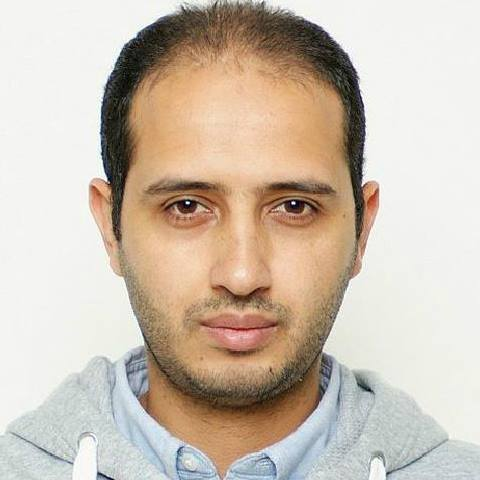
\includegraphics[width=0.19\columnwidth]{photo.jpg}}} \\
\href{http://eng.tanta.edu.eg/department/elc_comm/Mission.aspx}{Department of Electrical Engineering}    &                        \\
 \href{http://eng.tanta.edu.eg/} {Faculty of Engineering at Tanta University}    &                        \\
 \href{http://www.tanta.edu.eg/ar/index.aspx/}{Tanta University}                 &                        \\
Tanta, El Gharbeya Egypt     &                        \\
+201224058659    +8615603025014                        &                        \\
Tanta, El Gharbeya, Egypt - Postal Code:31521    &                        \\
\email{hossam.kasem@f-eng.tanta.edu.eg}          &  \\ 
\email{hossam.kasem@szu.edu.cn}      \\
\email{hossam.kasem@ejust.edu.eg}    \\
\email{hossamkasem1@gmail.com}    \\
\end{tabular}



\section{Research Interests}

 Machine Learning application in Digital Multimedia analysis.  Deep Learning applications for image Super resolution. Deep Learning application for Medical imaging. Applications of  Signal Processing in Wireless communications. Compressed Sensing applications in multimedia analysis. Audio and Multimedia compression. Applications of compressed sensing in wireless sensor network.\\


 




\section{Education}

\href{https://ejust.edu.eg/}{\textbf{Egypt-Japan University for Science and Technology (E-JUST)}},
Egypt
\begin{outerlist}

\item[] Ph.D.,
       % \href{http://www.sph.umn.edu/biostatistics/}%
             {School of Electronics, Communications and Computer Engineering},
              September  2015
              
              School of Electronics, Communications, and Computer Engineering
        \begin{innerlist}
        \item Thesis Title: \emph{Applications of Compressed Sensing in Multimedia and Wireless communication.}
        \item Advisors:
              \href{http://ecce.ejust.edu.eg/dr-maha-elsabrouty/}
                   {Maha Elsabrouty, Associate Professor} and
              \href{https://sites.google.com/a/ejust.kyushu-u.ac.jp/muta-e/}
                   {Osumu Muta, Associate Professor}
        \end{innerlist}
\end{outerlist}
\vspace{.1in}
\href{http://bu.edu.eg/}{\textbf{{Tanta University - Faculty of Enginerring }}},
Egypt
\begin{outerlist}
\item[] M.Sc.,
        \href{http://eng.tanta.edu.eg/}
             {Electrical Engineering},
             July. 2012
        \begin{innerlist}
        \item Topic: \emph { VHDL Implementation of Orthogonal Frequency Division multiplexing.}
        \item Advisor:
              \href{goo.gl/zrqcfY}
                   {Mohamed ُE. Nasr, Professor} and 
                   \href{goo.gl/t6jtgk}
                   {Fathi abdelsamie, Professor}
        \end{innerlist}
\href{http://eng.tanta.edu.eg//}{\textbf{{Tanta University - Faculty of Enginerring }}},
Egypt
\item[] B.Sc.,
        \href{http://eng.tanta.edu.eg/}
             {Electrical Engineering}, May 2004
        \begin{innerlist}
        \item Cumulative Grade: very Good (with honorary degree, rank the second).
        \item Graduation Project Grade: Excellent
        \item Cumulative Grade:Distinction with Honor(Percentage : 83.57\%, Equivalent GPA:3.71/4.0). Cumulatively ranked the 2nd in the Department of Electronics and Electrical Communication among 350 students.
        
        \end{innerlist}

\end{outerlist}

\section{Research Experience}

\textbf{Postdoctoral Research Fellow} \hfill {2017 to present \\}
\begin{innerlist}
\item[] \href{http://futuremedia.szu.edu.cn/People.aspx}{Research Institute for Future Media Computing}\\
		Faculty of Computer Science Software Engineering \\
         Shenzhen University\\
         Shenzhen - China\\
        Supervisor: Prof. \href{http://futuremedia.szu.edu.cn/peopleJianminJiang.aspx}{Jianmin Jiang} and \href{http://futuremedia.szu.edu.cn/peopleGuoweiHong.aspx}{Kwok-Wai Hung},  Ph.D \\  
\end{innerlist}

\textbf{Assistant Professor} \hfill {September  2015 to present}
\begin{innerlist}
\item[]Electronics and Electrical communications Dept.,\\
		Faculty of Enginerring \\
       Tanta University 
       
\end{innerlist}



\textbf{Research Assistant} \hfill { September 2014 to  June 2015}
\begin{innerlist}
\item[] \href{https://sites.google.com/a/ejust.kyushu-u.ac.jp/ejust_en/://research.nii.ac.jp/~prendinger/#}{Department of Advanced Information Technology },\\
       Kyushu University- Japan\\
       INTERNSHIP\\
        Supervisors: Osumu Muta, Ph.D .
\end{innerlist}

\textbf{Ph.D. Student} \hfill {September 2012 to September. 2015}
\begin{innerlist}
\item[] School of Electronics, Communications, and Computer Engineering,\\
		School of Electronics, Communications, and Computer Engineering\\
        Egypt Japan University of science and Technology (EJUST)\\
        Supervisors: Maha Elsabrouty, Ph.D and Osumu Muta, Ph.D.
\end{innerlist}

\textbf{Research Assistant and Teaching Assistance} \hfill {April. 2005 to September. 2012}
\begin{innerlist}
\item[] Electronics and Electerical communication Dept.,\\
Faculty of Enginerring \\
        Tanta University \\
        Supervisors:Mohamed E. Nasr, Ph.D and Fathi abdel samea, Ph.D.
\end{innerlist}

\section{Submitted Papers}
\vspace{0.1275in}

\begin{innerlist}


\item [\textbf{J1}] Jianmin Jiang, {\bf Hossam Kasem}, Kwok-Wai Hung ,\textquotedblleft Robust and Spatial-Transformed Deep Image Super-resolution (ST-DISR),\textquotedblright \emph{IEEE Transaction on Image Processing.}

\item [\textbf{C1}]  Jianmin Jiang, {\bf Hossam Kasem}  and Kwok-Wai Hung ,\textquotedblleft Efficient spectrum sensing technique base on energy detector compressive sensing and de-noising techniques,\textquotedblright \emph{IEEE  Conference on Computer Vision and Pattern Recognition (CVPR'2019) }


\item[\textbf{C2}] {\bf Hossam Kasem}, Jianmin Jiang, Kwok-Wai Hung ,\textquotedblleft STSR Robust Single Image Super-resolution via a Deep Spatial Transform,\textquotedblright \emph{ International Conference on Acoustics, Speech, and Signal Processing (ICAASP 2019).}
\end{innerlist}

\section{Recent Refereed Journal Publications}
\vspace{0.1275in}

\begin{innerlist}


\item [\textbf{J1}] Amr H. Hussien, {\bf Hossam Kasem},Mohamed A. Ezzat ,\textquotedblleft Efficient spectrum sensing technique base on energy detector compressive sensing and de-noising techniques,\textquotedblright \emph{International Journal of Engineering and  Technology,Vol. 46 (2017) No. 1 pp. 1-8.}


\item[\textbf{J2}]    Ibrahim Al-Nahhal, Ahmed Emran1, {\bf Hossam Kasem}, Adel B. Abd El-Rahman, Osamu Muta, Hiroshi Furukawa,\textquotedblleft Flexible fractional K-best sphere decoding for uncoded MIMO channels,\textquotedblright \emph{IEICE Communications Express,Vol. 4 (2015) No. 1 pp. 20-25.}
\end{innerlist}




















\section{Recent Refereed Conference Publications}
\vspace{.125in}
\begin{innerlist}
 
 
 \item[\textbf{C1}]  {\bf Hossam M. Kasem},  Kwok-Wai Hung and Jianmin Jiang,\textquotedblleft Image Super-Resolution Using Spatial Transform Network  \textquotedblright \emph{ International Conference on Pattern Recognition, ICPR, 2018}.\\


\item[\textbf{C2}]  {\bf Hossam M. Kasem}, Mohamed Al-Nahhal, Tawfik Ismail and Mohamed E. Nasr,\textquotedblleft FSO-SIMO System with SIM-DPSK over Log-normal Atmospheric Turbulence and Misalignment  \textquotedblright \emph{19th International Conference on Transparent Optical Networks (ICTON 2017)}.\\ 


\item[\textbf{C3}]  {\bf Hossam M. Kasem}, Osamu Muta, Maha Elsabrouty and Hiroshi Frukawa,\textquotedblleft Performance of Perceptual 1-Bit Compressed Sensing for Audio signal Compression \textquotedblright \emph{International Symposium on computer and communicationss,ISCC 
2015}.\\ 

\item[\textbf{C4}] {\bf Hossam M. Kasem}, Osamu Muta, Maha Elsabrouty and Hiroshi Frukawa,\textquotedblleft Quantized Perceptual Compressed Sensing for Audio signal Compression, \textquotedblright \emph{ Data Compression Conference,DCC 2015}.\\ 

\item[\textbf{C5}] {\bf Hossam M.Kasem},Maha El-Sabrouty,\textquotedblleft  The performance of One-bit Compressed Sensing with Perceptual Compressed Sensing for Audio Compression,\textquotedblright \emph { 
 Third International Japan-Egypt Conference on Electronics, Communications and Computers,2015.}\\
  
  
\item[\textbf{C6}] Adel B. Abd El-Rahman, Ibrahim Al-Nahhal, Ahmed Emran, {\bf Hossam Kasem },\textquotedblleft Fractional K-best Sphere Decoding Algorithm Over Rayleigh Fading MIMO Channels,\textquotedblright \emph { Second International Japan-Egypt Conference on Electronics, Communications and Computers,2014.}\\
  
\item[\textbf{C7}] {\bf Hossam M.Kasem},Maha El-Sabrouty,\textquotedblleft  A Comparative Study of Audio Compression Based on Compressed Sensing and Sparse Fast Fourier Transform (SFFT): Performance and Challenges,\textquotedblright \emph { 
International Symposium on Signal Processing and Information Technology IEEE ISSPIT 2013}  \\
 
 
 
\item[\textbf{C8}]  {\bf Hossam M Kasem}, Mohamed E Nasr, Amr H Hussein, \textquotedblleft A High Fidelity OFDM Image Communication System with Chaotic Maps,\textquotedblright \emph {
International Proceedings of Computer Science  Information Technology (ICIIP 2012).}\\


 \item[\textbf{C9}] Amr M Riad, Amr H Hussein, {\bf Hossam M Kasem}, Atef Abou El-Azm, \textquotedblleft A New Efficient Image Encryption Technique Based on Arnold and Idea Algorithms,\textquotedblright \emph {International Conference on Image and Infor-
mation Processing (ICIIP 2012).} \\
  
\item[\textbf{C10}] {\bf Hossam M Kasem}, Mohamed E Nasr, Elsayed A Sallam, FE Abd El-Samie,\textquotedblleft Efficient Transmission of 1D and 2D Chaotic Map Encrypted Images with Orthogonal Frequency Division Multiplexing,\textquotedblright \emph {Tenth International Symposium on Signal Processing and Information Technology (ISSPIT), 2010.}\\






\item[\textbf{C11}] {\bf Hossam M. Kasem}, Osamu Muta, Maha Elsabrouty and Hiroshi Frukawa,\textquotedblleft The Effect of One-bit Compressed Sensing on Audio Compression for Digital Communication Systems, 
 \textquotedblright \emph{ RCS, IEICE Technical Report,2015 }.\\ 

\item[\textbf{C12}]  {\bf Hossam M. Kasem}, Osamu Muta, Maha Elsabrouty and Hiroshi Frukawa,\textquotedblleft Performance of 1-bit Compressed Sensing for Audio Compression under AWGN Channel, \textquotedblright \emph{ RCS, IEICE Technical Report,2015}.\\ 

\item[\textbf{C13}]  {\bf Hossam M. Kasem}, Osamu Muta, Maha Elsabrouty and Hiroshi Frukawa,\textquotedblleft Cyclostationary Detection for Spectrum Sensing using Feature-Based Compressive Sensing, \textquotedblright \emph{ RCS, IEICE Technical Report,2015}.

\end{innerlist}


\section{Awards}





Scholarship from the Egyptian Ministry of Higher Education and Scientific Research
\begin{innerlist}
\item a Ph.D. program \hfill 2012--2015
\begin{innerlist}
    \item at E-JUST University (including 9-months in a Japanese University.
\end{innerlist}
\end{innerlist}

Postdoctoral 
\begin{innerlist}
\item Research Institute for Future Media Computing, Shenzhen University  \hfill 2017
\end{innerlist}

Best Paper Award 
\begin{innerlist}
\item Best paper awarded in JEC-EEC 2013 conference
\end{innerlist}


\section{Languages}

\begin{innerlist}
\item[] Engligh (TOFEL score 85.)\\
Arabic (Mother Tongue).

\end{innerlist}

\section{Presentations}
Statistical Meetings
\begin{innerlist}
\item ISSPIT Conference, Athens, Greece \hfill Dec. 2013
\item ISCC Conference, Cyprus, \hfill July 2015

\end{innerlist}

\halfblankline




\section{Teaching Experience}

%\textbf{Teaching Assistant} \hfill {Springs 2011--12}
Postgraduate-Assistant Professor\hfill {Summer 2015 to present}
\begin{innerlist}
\item[] Cryptography and Network Security \\
        Advanced Computer Networks \\
        Advanced Researches\\
        Information Security\\
        Machine Learning Algorithms \\
        Advanced Digital Signal Processing\\
\end{innerlist}

Undergraduate-Assistant Professor \hfill {Summer 2015 to present}
\begin{innerlist}

\item {\bf  Advanced Microprocessor.} Course, Faculty of Engineering, Higher Technological Institute. \hfill {\bf 2016}.\\

\item {\bf Microprocessor Interfacing .} Course, Faculty of Engineering, Higher Technological Institute. \hfill {\bf 2016}.\\

\item {\bf Introduction to microprocessor.} Course, Faculty of Engineering, Higher Technological Institute. \hfill {\bf 2016}.\\

\item {\bf Computer Security.} Course, Faculty of Engineering, Tanta University. \hfill {\bf 2016}.\\

\item {\bf Computer network.} Course, Faculty of Engineering, Tanta University. \hfill {\bf 2016}.\\

\item {\bf Computer and Network Security.} Course, Faculty of Engineering, Tanta University. \hfill {\bf 2015}.\\


\item {\bf Digital signal Processing.} Course, Faculty of Engineering, Tanta University. \hfill {\bf 2015}.\\


\item {\bf Eimage processing.} Course, Faculty of Engineering, Tanta University. \hfill {\bf 2015}.\\

\item {\bf Network Security .} Course, Faculty of Engineering, Tanta University. \hfill {\bf 2012}.\\

\item {\bf Communication laboratory.} Course, Faculty of Engineering, Tanta University. \hfill {\bf 2011}.\\

%\item {\bf Optical fiber laboratory.} Course, Faculty of Engineering, Tanta University. \hfill {\bf 2011}.\\


\item {\bf Network Security .} Course, Faculty of Engineering, Tanta University. \hfill {\bf 2011}.\\


\item {\bf Computer Technology .} Course, Faculty of Engineering, Tanta University. \hfill {\bf 2005}.\\

\item {\bf Electrical and Electronic measurements.} Course, Faculty of Engineering, Tanta University. \hfill {\bf 2010}.\\

\item {\bf Electrical and Electronic laboratory.} Course, Faculty of Engineering, Tanta University. \hfill {\bf 2010}.\\


\item {\bf Signal Processing course.} Course, Faculty of Engineering, Tanta University. \hfill {\bf 2009}.\\

\item {\bf Computer Technology .} Course, Faculty of Engineering, Tanta University. \hfill {\bf 2008}.\\


\item {\bf Modeling and Simulation .} Course, Faculty of Engineering, Tanta University. \hfill {\bf 2008}.\\

\item {\bf Pattern Recognition and Digital Image Processing .} Course, Faculty of Engineering, Tanta University. \hfill {\bf 2007}.\\

\item {\bf Computer and Network Security.} Course, Faculty of Engineering, Tanta University. \hfill {\bf 2006}.\\






%\item {\bf Spread Spectrum Communications.} Course, Faculty of Engineering, Tanta University. \hfill {\bf 2009}.\\

\item {\bf Digital Communications.} Course, Faculty of Engineering, Tanta University. \hfill {\bf 2009}.\\

\item {\bf Computer Networks.} Course, Faculty of Engineering, Tanta University. \hfill {\bf 2009}.\\


\item {\bf Compilers} Course, Faculty of Engineering, Tanta University. \hfill {\bf 2008}.\\

\item {\bf Digital Electronics.} Course, Faculty of Engineering, Tanta University. \hfill {\bf 2007}.\\

\item {\bf Digital Electronics.} Course, Faculty of Engineering, Tanta University. \hfill {\bf 2006}.\\


%\item {\bf Basic and advanced course of analog communications.} Course, Faculty of Engineering, Tanta University. \hfill {\bf 2006}.\\

%\item {\bf Basic and advanced course of digital communications.} Course, Faculty of Engineering, Tanta University. \hfill {\bf 2006}.\\


%\item {\bf Advanced course of Electronic circuits.} Course, Faculty of Engineering, Tanta University. \hfill {\bf 2005}.\\
        
\end{innerlist}

\section{Service}

\begin{innerlist}
    \item Judging Committee of Egyptian Engineering Day \hfill {Sep. 2016} \\
     The Egyptian Engineering Day is an annual summit that facilitates the opportunity for the best engineers to present and fully explain their projects to the elite members of engineering field from all over Egypt.
    
    \item The committee of updating the postgraduate bylaw for the Faculty of Engineering, Tanta  University.
\item IThe committee of Quality assurance, Tanta University. 
%\item IPIN'2011 student travel grant.  \\
\item IEEE signal processing society . 
 \item Member of Technical program committee for JECEEC conference(2015 to Present).
  \item Reviewer for IEEE Transactions on  Image Signal Processing Transaction Journal.
   \item Reviewer for EuraSip Transaction Journal.
    
\end{innerlist}




\section{General Skills}
\begin{innerlist}
\item[] Effective Research and Development Capabilities\\
  Efficient Algorithms Design and Implementation\\
  Code Optimization for Resources and Performance\\
    Team Player with Leadership, Conflict Management, and Problem Solving Capabilities
\end{innerlist}

\begin{comment}
\section{Hardware and Software Skills}
Computer Programming:

\begin{innerlist}
    \item C, C$+$$+$, Java, JavaScript, Pascal, PHP,
        Lisp, UNIX shell scripting, GNU make,
        AppleScript, SQL, MySQL, \Matlab, Mathematica, and others
\end{innerlist}
\end{comment}


\end{document}

%%%%%%%%%%%%%%%%%%%%%%%%%% End CV Document %%%%%%%%%%%%%%%%%%%%%%%%%%%%%

%----------------------------------------------------------------------%
% The following is copyright and licensing information for
% redistribution of this LaTeX source code; it also includes a liability
% statement. If this source code is not being redistributed to others,
% it may be omitted. It has no effect on the function of the above code.
%----------------------------------------------------------------------%
% Copyright (c) 2007, 2008, 2009, 2010, 2011 by Theodore P. Pavlic
%
% Unless otherwise expressly stated, this work is licensed under the
% Creative Commons Attribution-Noncommercial 3.0 United States License. To
% view a copy of this license, visit
% http://creativecommons.org/licenses/by-nc/3.0/us/ or send a letter to
% Creative Commons, 171 Second Street, Suite 300, San Francisco,
% California, 94105, USA.
%
% THE SOFTWARE IS PROVIDED "AS IS", WITHOUT WARRANTY OF ANY KIND, EXPRESS
% OR IMPLIED, INCLUDING BUT NOT LIMITED TO THE WARRANTIES OF
% MERCHANTABILITY, FITNESS FOR A PARTICULAR PURPOSE AND NONINFRINGEMENT.
% IN NO EVENT SHALL THE AUTHORS OR COPYRIGHT HOLDERS BE LIABLE FOR ANY
% CLAIM, DAMAGES OR OTHER LIABILITY, WHETHER IN AN ACTION OF CONTRACT,
% TORT OR OTHERWISE, ARISING FROM, OUT OF OR IN CONNECTION WITH THE
% SOFTWARE OR THE USE OR OTHER DEALINGS IN THE SOFTWARE.
%----------------------------------------------------------------------%
